\section{Absorption of Rb resonance radiation by atomic Rb}

\subsection{Experimental principle}
The Beer--Lambert law relates the transmitted intensity to the Rb number
density $\rho$ through
\begin{equation}
  I(\rho) = I_0\,e^{-\sigma\rho L} + I_{\mathrm{bg}},
  \label{eq:beer_lambert}
\end{equation}
where $L$ is the cell length, $\sigma$ the effective absorption cross
section averaged over the lamp profile, and $I_{\mathrm{bg}}$ the
non-resonant background observed at the optically thick limit
(Eq.~2C-2 of Ref.~\cite{OpticalPumpingRubidium2002}). Since $\rho(T)$
obeys an Arrhenius-like vapor-pressure law, mapping the cell temperature
onto $\rho$ and fitting $\ln(I-I_{\mathrm{bg}})$ against $\rho$ yields
$\sigma$ directly from the slope.

\subsection{Settings}
The linear polariser and quarter-wave plate were removed so that the full
D$_1$+D$_2$ lamp intensity reached the detector (CH1). With the electronic
chain as described in Section~\ref{sec:common_procedure}, the cell was
cycled through three thermal sweeps: Run~1 (heating, \SIrange{50}{80}{\celsius},
16 points), Run~2 (cooling, \SIrange{28}{80}{\celsius}, 26 points), and
Run~3 (re-heating, \SIrange{60}{80}{\celsius}, 11 points), in each case in
\SI{2}{\celsius} increments once the thermistor had stabilised. A room-temperature
reference ($V_0$ at \SI{20.8}{\celsius}) fixed the zero-density baseline, and
three readings per set-point were combined as Type~A/Type~B $u$-values with
the \SI{0.01}{\volt} meter resolution~\cite{OpticalPumpingRubidium2002}.

\subsection{Atomic number-density interpolation}
Table~4A-1 of Ref.~\cite{OpticalPumpingRubidium2002} tabulates $\rho(T)$ on a
\SI{10}{\kelvin} grid while our set-points are spaced by \SI{2}{\celsius}. We
therefore interpolate $\ln\rho$ linearly in $T$ rather than $\rho$ directly,
preserving the Arrhenius character of the vapor-pressure curve and avoiding
the bias that linear interpolation in $\rho$ would introduce. The resulting
densities span $\rho \in [\SI{4e15}{}, \SI{2e18}{}]\,\si{atoms\per\meter\cubed}$.

\subsection{Beer--Lambert analysis}
Subtracting the saturation-plateau background
$I_{\mathrm{bg}} = 0.2400(50)\,\si{\volt}$ (fixed from the $T \gtrsim
  \SI{78}{\celsius}$ data, where the lamp wing and buffer-gas emission
dominate) linearises Eq.~\ref{eq:beer_lambert}:
\begin{equation}
  \ln\bigl(I-I_{\mathrm{bg}}\bigr) = \ln I_0 - \sigma L\,\rho,
  \label{eq:ln_fit}
\end{equation}
with $L = 2.500(29)\,\si{\centi\meter}$. To exclude the saturated tail we
restrict the weighted regression to $\rho < \SI{2.0e17}{atoms\per\meter\cubed}$
and extract $\sigma = -\mathrm{slope}/L$. Figure~\ref{fig:4a_beer_lambert}
overlays the three fits, and Table~\ref{tab:4a_sigma} gives the parameters.

\begin{figure}[ht]
  \centering
  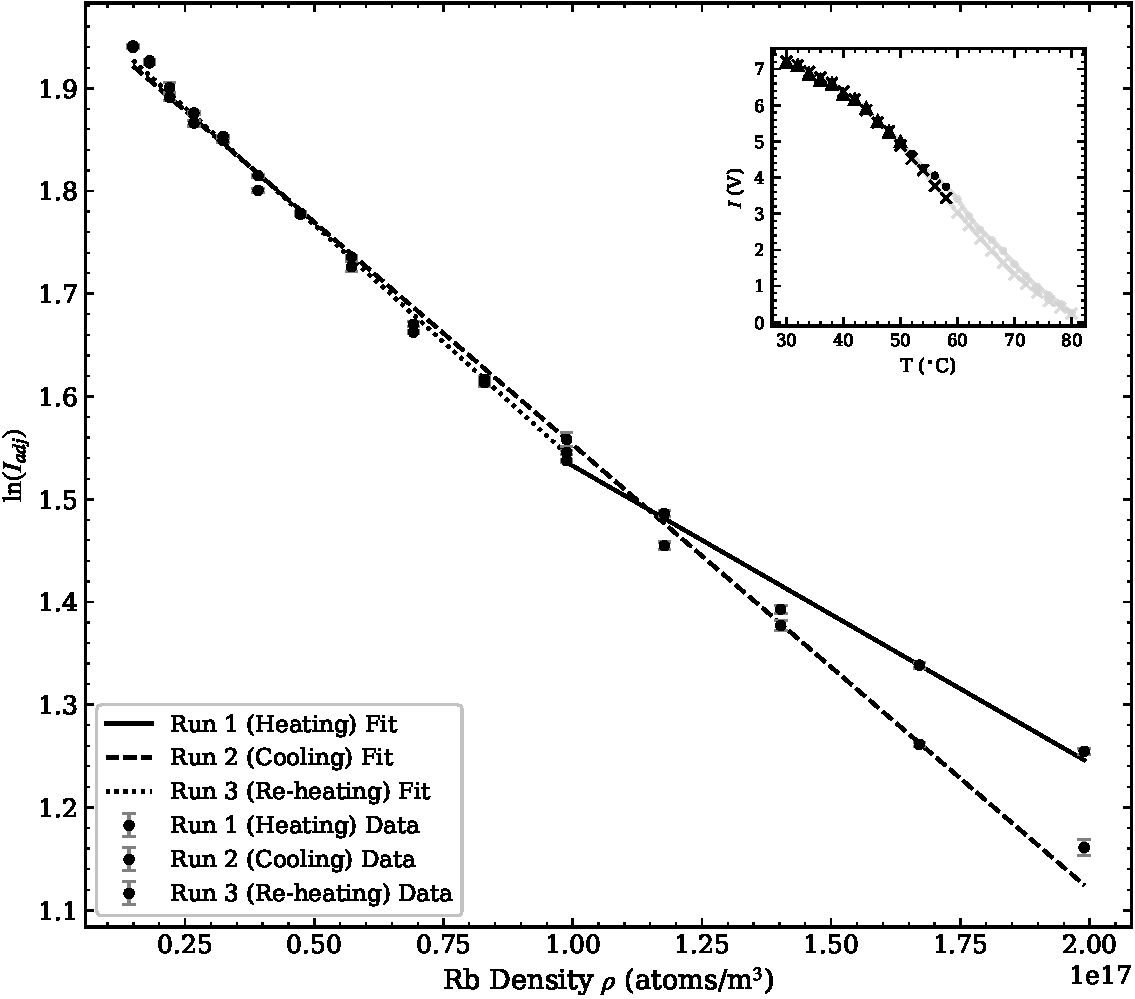
\includegraphics[width=0.72\linewidth]{figures/4a_Combined_Fit_Hysteresis.pdf}
  \caption{Linearised Beer--Lambert fit, $\ln(I-I_{\mathrm{bg}})$ vs.\ Rb
    number density, for all three sweeps. Only points with
    $\rho < \SI{2e17}{atoms\per\meter\cubed}$ enter each fit (filled markers);
    the rest lie on the optically thick plateau. Inset: photodetector
    voltage vs.\ temperature, showing the heating/cooling hysteresis that
    dominates the run-to-run spread.}
  \label{fig:4a_beer_lambert}
\end{figure}

\begin{table}[ht]
  \centering
  \caption{Beer--Lambert fit results. Slope is in $10^{-18}\,\si{\meter\squared\per atom}$ and the cross section in $10^{-16}\,\si{\meter\squared}$.}
  \label{tab:4a_sigma}
  \begin{tabular}{lccc}
    \toprule
    Run                & Points used & Slope ($10^{-18}\,\mathrm{m^2/atom}$) & $\sigma$ ($10^{-16}\,\mathrm{m^2}$) \\
    \midrule
    Run~1 (heating)    & 5/16        & $-2.894(33)$                          & $1.158(19)$                         \\
    Run~2 (cooling)    & 15/26       & $-4.331(23)$                          & $1.732(22)$                         \\
    Run~3 (re-heating) & 11/11       & $-4.564(50)$                          & $1.825(29)$                         \\
    \bottomrule
  \end{tabular}
\end{table}

The three runs bracket $\sigma \simeq (1.2\text{--}1.8)\times 10^{-16}\,\si{\meter\squared}$.
Run~1 is pulled toward zero because heating starts with a cold cell in
which Rb has condensed onto the walls: the vapor density lags the
tabulated equilibrium curve until the cell re-saturates, so $\rho$ is
systematically overestimated at a given $T$ and the inferred slope (hence
$\sigma$) is biased low. Runs~2 and~3 start from a thoroughly equilibrated
hot cell and are mutually consistent within ${\sim}2\sigma$.

\subsection{Thermal hysteresis}
Table~\ref{tab:4a_hysteresis} tabulates the heating/cooling disagreement at
common temperatures; the $T$--$I$ inset of Fig.~\ref{fig:4a_beer_lambert}
shows the trend. The deviation is monotonic in $T$: $<1\%$ at
\SI{50}{\celsius}, $\sim 10\%$ at \SI{60}{\celsius}, peaks near $22\%$
around \SIrange{76}{78}{\celsius}, then collapses at \SI{80}{\celsius} once
both runs reach the optically thick plateau. The kinetic cause is rubidium exchange between the glass walls and
the vapor: heating must first evaporate Rb off the walls before $\rho(T)$
reaches Table~4A-1, whereas cooling produces the opposite lag as atoms
recondense. Because Table~4A-1 assumes \emph{equilibrium} saturated vapor,
any such deviation violates the $T \mapsto \rho$ mapping and directly
inflates the spread in $\sigma$. Run~1 is therefore discarded from the
best-estimate average, and the weighted mean of Runs~2 and~3 gives
\begin{equation}
  \sigma_{\mathrm{exp}} = 1.766(50)\times 10^{-16}\,\si{\meter\squared},
  \label{eq:sigma_best}
\end{equation}
where the uncertainty includes the run-to-run scatter as a systematic
contribution.

\begin{table}[ht]
  \centering
  \caption{Transmitted intensity at temperatures common to Run~1 and Run~2,
    with fractional difference $\Delta I/I_{\mathrm{heat}}$.}
  \label{tab:4a_hysteresis}
  \begin{tabular}{cccc}
    \toprule
    $T$ (\si{\celsius}) & $I_{\mathrm{heat}}$ (V) & $I_{\mathrm{cool}}$ (V) & $\Delta I/I_{\mathrm{heat}}$ \\
    \midrule
    50                  & 4.930                   & 4.893                   & $0.7\%$                      \\
    56                  & 4.053                   & 3.770                   & $7.0\%$                      \\
    60                  & 3.407                   & 3.043                   & $10.7\%$                     \\
    66                  & 2.267                   & 1.980                   & $12.6\%$                     \\
    70                  & 1.600                   & 1.323                   & $17.3\%$                     \\
    76                  & 0.751                   & 0.588                   & $21.8\%$                     \\
    78                  & 0.513                   & 0.400                   & $22.0\%$                     \\
    80                  & 0.249                   & 0.244                   & $2.3\%$                      \\
    \bottomrule
  \end{tabular}
\end{table}

\subsection{Comparison with theory}
The resonant cross section at line centre is given by Eq.~2C-4 of
Ref.~\cite{OpticalPumpingRubidium2002},
\begin{equation}
  \sigma_0 = \frac{2}{\Delta\nu_D}\cdot\frac{\lambda_0^2\,g_2}{8\pi\,g_1}\cdot\frac{1}{\tau},
  \qquad \Delta\nu_D = 3\times 10^{-20}\,\nu_0\sqrt{T/M}.
  \label{eq:sigma0_theory}
\end{equation}
Using the D$_1$ parameters $\lambda_0 = \SI{794.98}{\nano\meter}$,
$\tau = \SI{27.7}{\nano\second}$, $g_1=g_2=2$ at our mean operating
temperature $T \simeq \SI{333}{\kelvin}$ gives
$\Delta\nu_D \simeq \SI{0.5}{\giga\hertz}$ and
$\sigma_0 \simeq 1.5\times 10^{-15}\,\si{\meter\squared}$, reduced to
${\sim}1\times 10^{-15}\,\si{\meter\squared}$ once the finite lamp width
and hyperfine overlap are accounted for. Our measured value
(Eq.~\ref{eq:sigma_best}) is thus a factor ${\sim}6\text{--}8$ smaller
than this peak $\sigma_0$: the lamp emits a broad self-reversed profile
that overlaps the Rb Doppler absorption line only partially. The same
factor-of-10 reduction appears in the sample analysis of
Ref.~\cite{OpticalPumpingRubidium2002}
($\sigma \simeq 1.6\times 10^{-16}\,\si{\meter\squared}$), so our result
agrees with published measurements on this apparatus class. For
orientation, the geometric cross section
$\sigma_{\mathrm{geom}} = \pi r_{\mathrm{Rb}}^2 \simeq 1.9\times
  10^{-19}\,\si{\meter\squared}$ (using $r_{\mathrm{Rb}} \simeq
  \SI{2.48e-10}{\meter}$) is three orders of magnitude below
$\sigma_{\mathrm{exp}}$: resonant photon--atom interaction is controlled
by the dipole oscillator strength, not by atomic size, as discussed in
§2C of Ref.~\cite{OpticalPumpingRubidium2002} and
§4 of Ref.~\cite{OPTOpticalPumping2024}.

\subsection{Uncertainty budget and operating-point choice}
The dominant error in $\sigma_{\mathrm{exp}}$ is \emph{systematic}: the
Table~4A-1 density curve itself carries an uncertainty of order tens of
percent over our range~\cite{OpticalPumpingRubidium2002}, and the
wall-equilibration hysteresis discussed above adds another ${\sim}10\%$ at
our dwell times. Photodetector shot-to-shot scatter
(\SI{10}{\milli\volt}) and path-length uncertainty ($<2\%$) are
subdominant, so future improvements should replace Table~4A-1 with an
independent density calibration (e.g.\ integrated absorption of a
narrow-linewidth laser) rather than refine the photometric readout. The
same analysis also fixes a useful operating window for the subsequent
experiments: below ${\sim}\SI{50}{\celsius}$ the optical depth is too low
to produce a strong pumping signal, while above ${\sim}\SI{70}{\celsius}$
the cell saturates at the non-resonant background. We therefore operate
the ODMR (Section~\ref{sec:4b}) and transient (Section~\ref{sec:4d})
measurements at $T \approx \SI{50}{\celsius}$, in line with §6.3 of
Ref.~\cite{OPTOpticalPumping2024}.
